\documentclass[12pt]{article}
\usepackage[utf8]{inputenc}
\usepackage[T1]{fontenc}
\usepackage{indentfirst}
\usepackage{amsmath}
\usepackage{amssymb}
\usepackage{natbib}
\usepackage{graphicx}
\usepackage{float}
\usepackage[a4paper, margin = 2 cm]{geometry}
\usepackage{fancyhdr}
\usepackage{wrapfig}
\usepackage{hyperref}

\title{SK projekt 3}
\author{Dominik Wawszczak}
\date{2023-06-08}

\begin{document}
	\setlength{\parindent}{0 cm}
	
	Dominik Wawszczak \hfill Sieci Komputerowe
	
	numer indeksu: 440014 \hfill Projekt 3
	
	numer grupy: 2
	
	\bigskip
	\hrule
	\bigskip
	
	Na poniższym rysunku przedstawiono logiczne połączenie ruterów \texttt{R11},
	\texttt{R12}, \texttt{R13} i \texttt{R14}.
	\begin{center}
		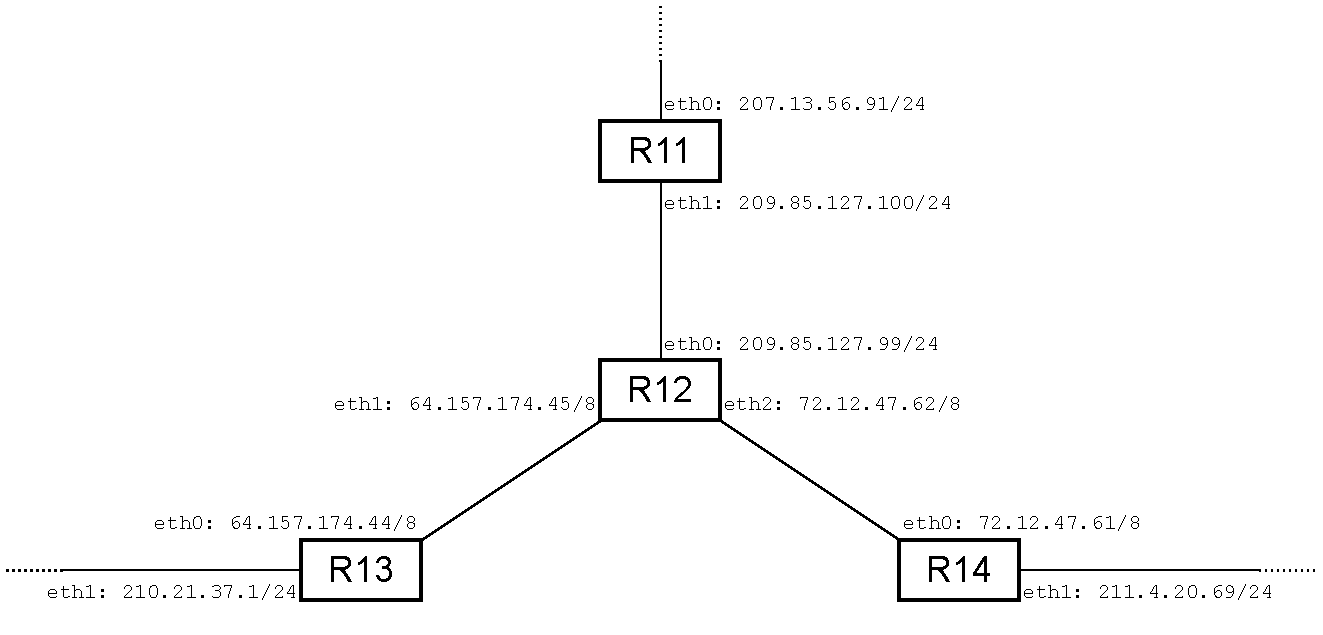
\includegraphics[width = 0.95 \textwidth]{./routers-image.pdf}
	\end{center}
	
	\medskip
	
	Poniżej przedstawiono fragment tablicy tras rutera \texttt{R12}.
	\begin{center}
		\begin{tabular}{|c|c|c|c|}
			\hline
			Cel & Maska & Interfejs & Brama \\
			\hline
			\hline
			\texttt{209.85.127.0} & \(24\) & \texttt{eth0} & \texttt{0.0.0.0} \\
			\hline
			\texttt{207.13.56.0} & \(24\) & \texttt{eth0} & \texttt{209.85.127.100} \\
			\hline
			\texttt{222.67.1.0} & \(24\) & \texttt{eth0} & \texttt{209.85.127.100} \\
			\hline
			\texttt{64.0.0.0} & \(8\) & \texttt{eth1} & \texttt{0.0.0.0} \\
			\hline
			\texttt{210.21.37.0} & \(24\) & \texttt{eth1} & \texttt{64.157.174.44} \\
			\hline
			\texttt{25.0.0.0} & \(8\) & \texttt{eth1} & \texttt{64.157.174.44} \\
			\hline
			\texttt{72.0.0.0} & \(8\) & \texttt{eth2} & \texttt{0.0.0.0} \\
			\hline
			\texttt{211.4.20.0} & \(24\) & \texttt{eth2} & \texttt{72.12.47.61} \\
			\hline
			\texttt{193.19.88.0} & \(24\) & \texttt{eth2} & \texttt{72.12.47.61} \\
			\hline
		\end{tabular}
	\end{center}
	
	\medskip
	
	Wynik polecenia \texttt{traceroute pigeon.zad3sik.edu.pl} z komputera
	\texttt{eagle.zad3sik.edu.pl}:
	\begin{verbatim}
		1 * * *
		2 * * *
		3 R13.zad3sik.edu.pl (210.21.37.1)
		4 R12.zad3sik.edu.pl (64.157.174.45)
		5 R11.zad3sik.edu.pl (209.85.127.100)
		6 * * *
		7 * * *
		8 * * *
		9 * * *
		10 * * *
		11 * * *
		12 * * *
		13 pigeon.zad3sik.edu.pl (222.67.1.27)
	\end{verbatim}
	
	\medskip
	
	Wynik polecenia \texttt{traceroute pigeon.zad3sik.edu.pl} z komputera
	\texttt{kestrel.zad3sik.edu.pl}:
	\begin{verbatim}
		1 * * *
		2 * * *
		3 * * *
		4 * * *
		5 * * *
		6 R14.zad3sik.edu.pl (211.4.20.69)
		7 R12.zad3sik.edu.pl (72.12.47.62)
		8 R11.zad3sik.edu.pl (209.85.127.100)
		9 * * *
		10 * * *
		11 * * *
		12 * * *
		13 * * *
		14 * * *
		15 * * *
		16 pigeon.zad3sik.edu.pl (222.67.1.27)
	\end{verbatim}
	
	\medskip
	
	Zawartość pliku \texttt{zad3sik.edu.pl}:
	\begin{verbatim}
		$TTL    1h
		@   IN  SOA ns1.zad3sik.edu.pl. root.zad3.edu.pl. (
		        1       ; Serial
		        604800  ; Refresh
		        86400   ; Retry
		        2419200 ; Expire
		        604800) ; Negative Cache TTL
		
		            IN  NS  ns1.zad3sik.edu.pl.
		            IN  NS  ns2.zad3sik.edu.pl.
		
		ns1         IN  A   142.27.28.98
		ns2         IN  A   142.27.28.99
		
		pigeon      IN  A   222.67.1.27
		eagle       IN  A   25.3.143.12
		kestrel     IN  A   193.19.88.91
		
		R11-eth0    IN  A   207.13.56.91
		R11-eth1    IN  A   209.85.127.100
		
		R12-eth0    IN  A   209.85.127.99
		R12-eth1    IN  A   64.157.174.45
		R12-eth2    IN  A   72.12.47.62
		
		R13-eth0    IN  A   64.157.174.44
		R13-eth1    IN  A   210.21.37.1
		
		R14-eth0    IN  A   72.12.47.61
		R14-eth1    IN  A   211.4.20.69
	\end{verbatim}
\end{document}
